\section{Posición de reposo}

La posición de reposo de la excavadora es la siguiente:

% foto de la posición de la excavadora
\begin{figure}[H]
    \centering
    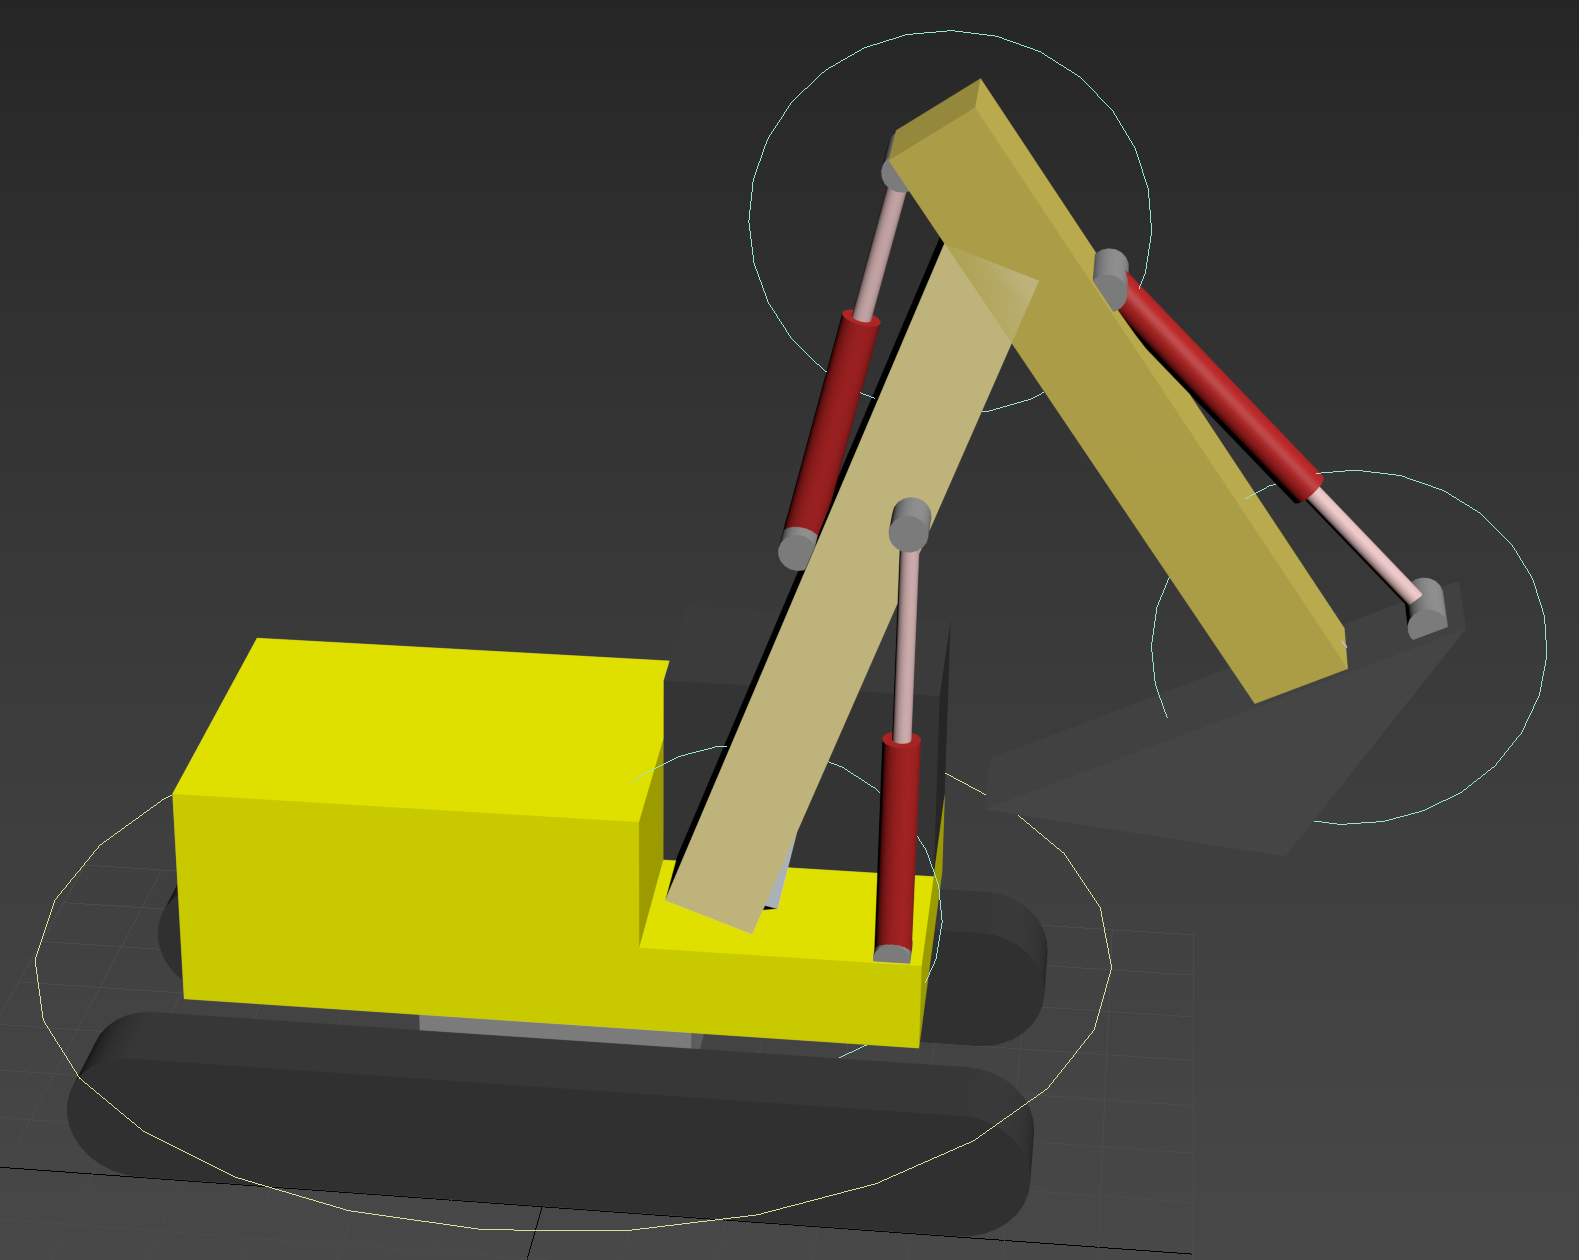
\includegraphics[width=0.5\textwidth]{imagenes/idle.png}
    \caption{Posición de reposo de la excavadora.}
 \end{figure}

 Como se puede observar, es muy similar a la posición que tienen las excavadoras en la vida real, con el brazo levantado para poder moverse libremente.

 \bigskip

Para realizar el \textit{Freeze Transform}, he seleccionado todo el modelo, salvo los \textit{sliders} y los pistones, ya que la posición de reposo eliminaba el \textit{LookAt Constraint} de los pistones.

\bigskip

Cabe destacar que se podría haber hecho la posición de reposo a los pistones también, añadiendo el controlador de nuevo, pero no he llegado a conseguir que funcione del todo bien, por lo que lo he dejado así.

\bigskip
\newpage

La única desventaja que tiene esta configuración es que al elegir \textit{Transform To Zero}, aparecerán varias veces el siguiente error:

% foto del error
\begin{figure}[H]
    \centering
    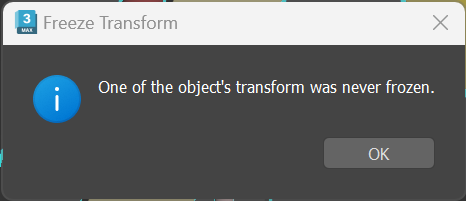
\includegraphics[width=0.5\textwidth]{imagenes/error.png}
    \caption{Ventana de error al volver a la posición de reposo.}
 \end{figure}

Esto es debido a que los pistones no tienen posición congelada, de forma que el programa avisa de lo sucedido.